%!TEX root = start.TEX

%----------------Resultados de la tesis----------


\section{Resultados de la tesis}

\frame{
\begin{block}
{\Large{Resultados de la tesis}}
\end{block}
%\vskip 0.5cm
\begin{itemize}
	\item<1->Indicadores:
	\begin{itemize}
	\item Efectividad(Prop. Verdaderos Pos): {$PVP= \frac{Verdaderos\,Positivos}{{Verdaderos\,Positivos} + {Falsos\,Negativos}}$}
	\vskip 0.2cm
	\item Especificidad(Prop. Verdaderos Neg): {$PVN= \frac{Verdaderos\,Negativos}{{Verdaderos\,Negativos} + {Falsos\,Positivos}}$}
	\vskip 0.2cm
	\item Valor Predictivo Positivo (Precisión): {$PPV = \frac{Verdaderos\,Positivos}{{Verdaderos\,Positivos}+{Falsos\,Positivos}}$}
	\vskip 0.2cm
	\item Acuracia (Exactitud): {$ACC= \frac{Verdaderos\,Positivos+Verdaderos\,Negativos}{Total\,de\,Imagenes}$}
	\end{itemize}
	\vskip 0.2cm	
	\item<2->Donde:
	\begin{itemize}
		\item[--] Verdaderos Positivos: Imágenes correctamente indentificadas.
		\item[--] Falsos Positivos: Imágenes incorrectamente identificadas.
		\item[--] Verdaderos Negativo:Imágenes correctamente rechazadas.
		\item[--] Falsos Negativos:Imágenes incorrectamente rechazadas.
	\end{itemize}
	
\end{itemize}
}

\frame{
\begin{block}
{\Large{Resultados de la tesis}}
\end{block}
%\vskip 0.5cm
\begin{itemize}
	\item<1->Utilizando los anteriores indicadores, podemos obtener dos más:
	\begin{itemize}
		\item Curvas ROC : Relación entre Efectividad y Especificidad
		\vskip 0.2cm	
		\item Curvas PR  : Relación entre Precisión y Efectividad(Recall)
		\vskip 0.2cm	
	\end{itemize}
	\vskip 0.3cm
	\item<2->Ambas curvas se utilizan normalmente para estudiar la salida de un clasificador. En las Curvas ROC un aumento en la sensibilidad está acompañado por un decremento en la especificidad. Esto significa que la esquina superior izquierda del gráfico es el punto ideal, debido a que muestran la relación entre las muestras clasificadas adecuadamente (\textit{Proporción de Verdaderos Positivos} - PVP) y las muestras que no pertenecen a la clase pero se clasificaron como si lo fueran (\textit{Proporción de Falsos Positivos - PFP}).

	%La curva que más se acerque a la diagonal de 45 grados en el espacio ROC, es la prueba menos acertada.
\end{itemize}
}

\frame{
\begin{block}
{\Large{Resultados de la tesis}}
\end{block}
%\vskip 0.5cm
\begin{itemize}
	\item<1->De manera similar, las Curvas PR (\textit{Precision -Recall}) representan la relación entre la Efectividad y Precisión del clasificador. El objetivo es tener un modelo que se posicione en la esquina superior derecha, que básicamente consiste en obtener solo los positivos verdaderos sin falsos positivos ni falsos negativos: un clasificador perfecto. En la situación en la que se tiene clases con cantidades no balanceadas, como es el caso del Dataset- Perú, a menudo es más útil utilizar el Área bajo la Curva PR como indicador del clasificador, \citep{Davis-2006-RPR-1143844-1143874}.
	
	\item<2->El mejor sistema de clasificación es el que produce un conjunto de clasificadores que maximice el área bajo la curva(AUC - Area Under the Curve)\citep{SandovalCereza}.

\end{itemize}
}

%------------------------------------------------------------------------------------------------------------------------------------------

\frame{
\begin{block}
{\Large{Resultados de la tesis - Señales de Tránsito de Alemania}}
\end{block}
%\vskip 0.5cm

	\begin{table}[H]
			\begin{center}
			\caption{\small{Indicadores de los 5 modelos entrenados para el Dataset - Alemania}}
			\setlength{\tabcolsep}{2pt}
			\begin{tabular}{|>{\tiny}c|>{\tiny}c|>{\tiny}c|>{\tiny}c|>{\tiny}c|>{\tiny}c|}
			
			\cline{1-6}
			\textbf{Indicadores}    &  \textbf{Modelo A(\%)} & \textbf{Modelo B(\%)} & \textbf{Modelo C(\%)} &\textbf{ Modelo D(\%)} & \textbf{Modelo E(\%)} \\ \hline
			\multicolumn{1}{|c|}{\textbf{\tiny PVP}}        & 96.14     & 98.35       & 98.08       & 98.37       & 98.61       \\ \hline
			\multicolumn{1}{|c|}{\textbf{\tiny PVN}}        & 99.93     & 99.96       & 99.96       & 99.96       & 99.97       \\ \hline
			\multicolumn{1}{|c|}{\textbf{\tiny PPV}}        & 95.69     & 97.52       & 97.57       & 97.78       & 98.01      \\ \hline
			\multicolumn{1}{|c|}{\textbf{\tiny AUC-PR}}     & 94.31     & 96.88       & 96.60       & 96.93       & 97.30       \\ \hline
			\multicolumn{1}{|c|}{\textbf{\tiny AUC-ROC}}    & 98.04     & 99.15       & 99.02       & 99.17       & 99.29       \\ \hline
			\multicolumn{1}{|c|}{\textbf{\tiny ACC}}        & 97.08     & 98.41       & 98.27       & 98.43       & 98.62       \\ \hline
			\end{tabular}
			\end{center}
		\end{table}
}



\frame{
\begin{block}
{\Large{Señales de Tránsito de Alemania}}

\end{block}
%\vskip 0.5cm

	\begin{figure}[H]
		\begin{center}
		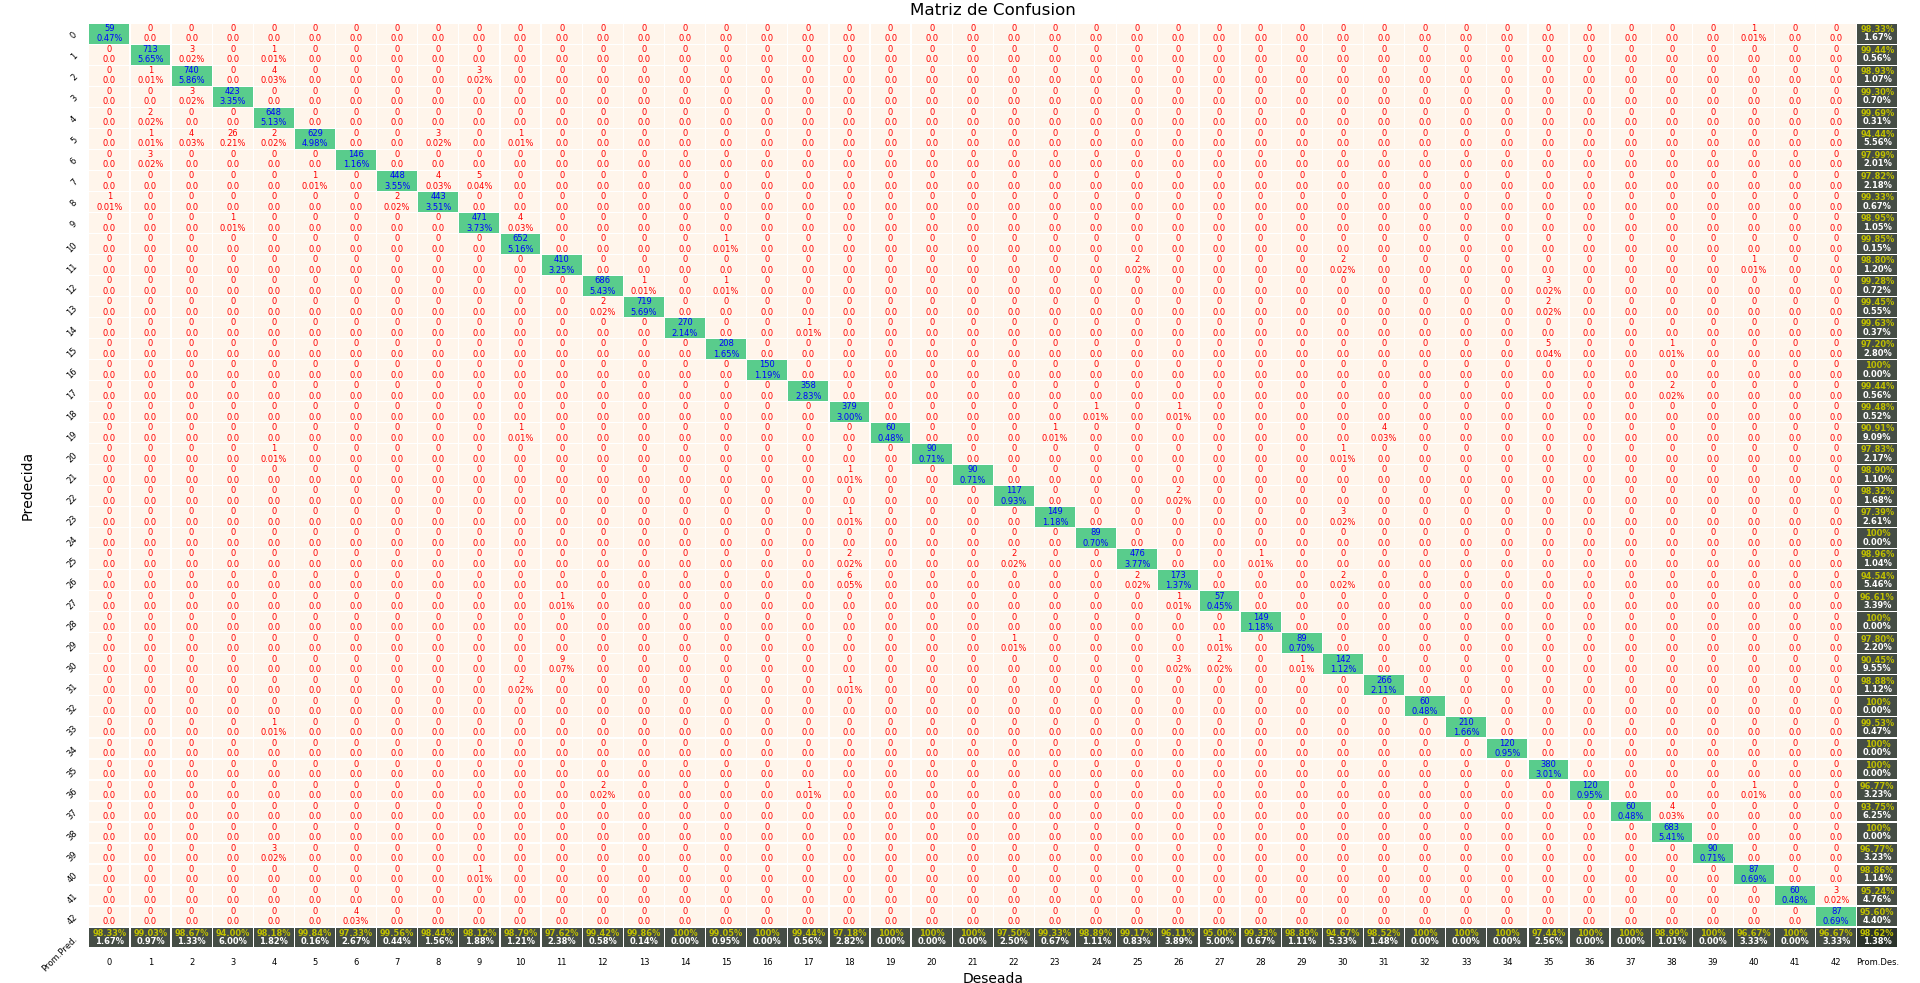
\includegraphics[width=\textwidth, height=1.2\textheight,keepaspectratio]{images/desarrollo/testResults/german/model_A_A_1} 
		\end{center}
		\begin{center}
		\caption{\tiny{Matriz de Confusión del Modelo E - Dataset de imágenes de Alemania}}
		\vspace{-1em}
		{\tiny {Fuente: Elaboración propia}}
		\end{center}
		%\vspace{-1.5em}
	\end{figure}
}


\frame{
\begin{block}
{\Large{Señales de Tránsito de Alemania}}

\end{block}

	\begin{figure}[H]
		\begin{center}
		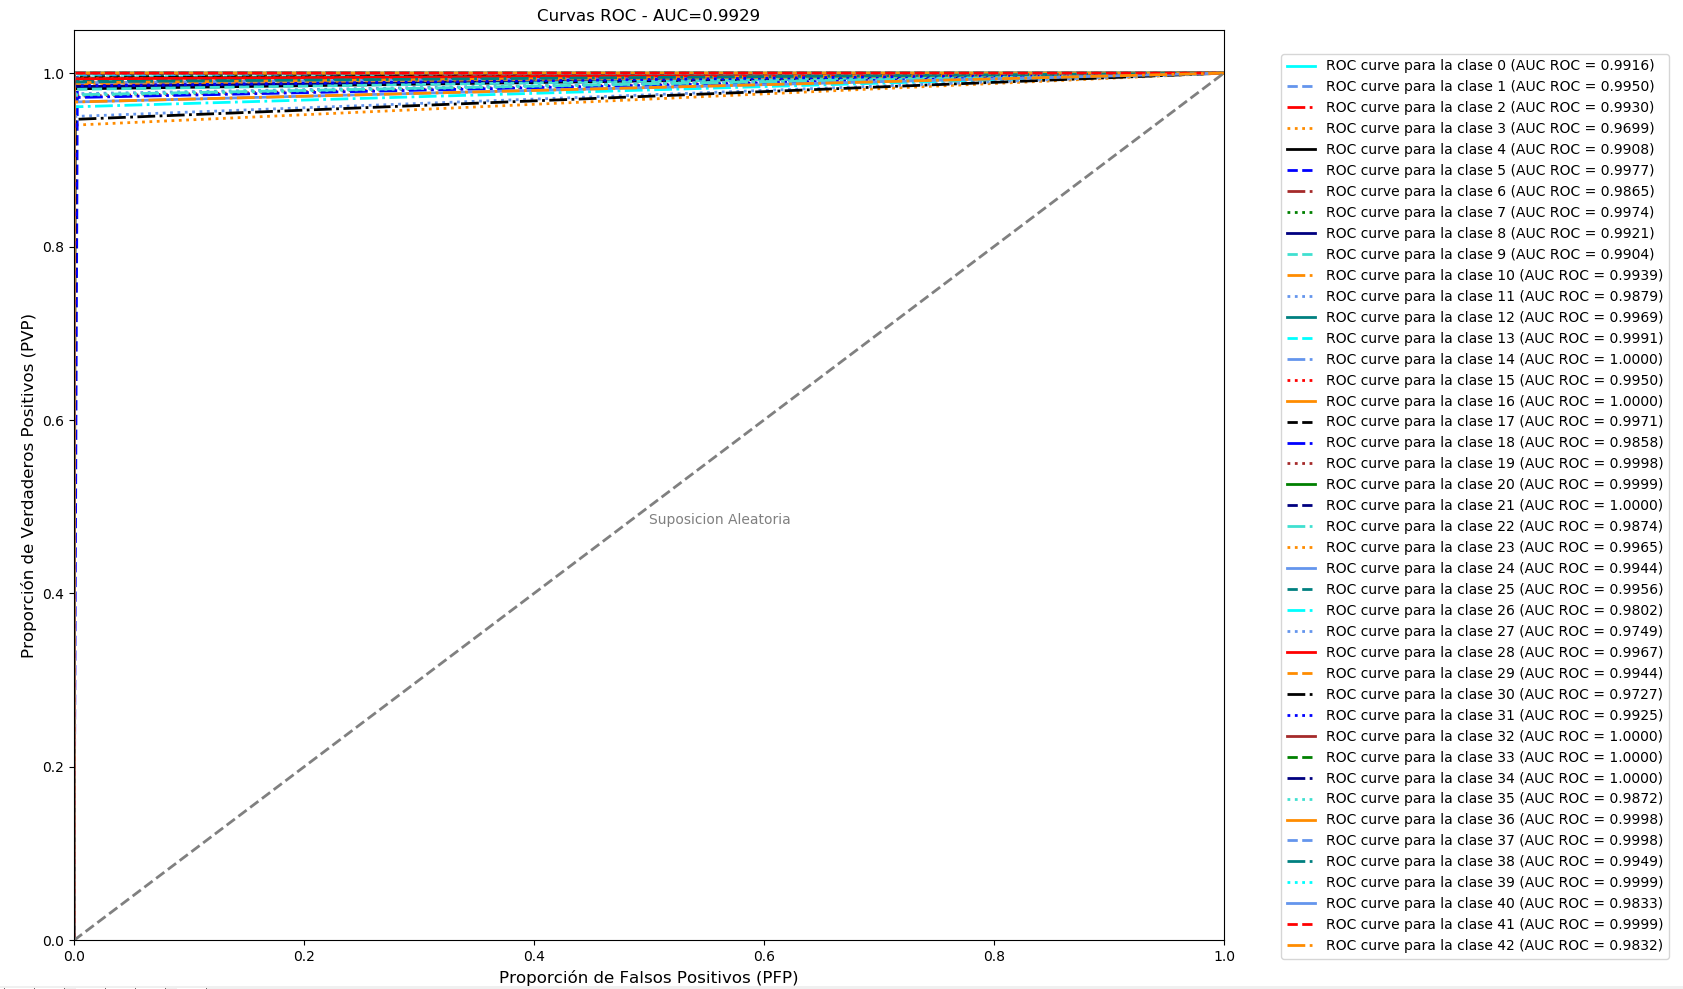
\includegraphics[width=\textwidth, height=0.7\textheight,keepaspectratio]{images/desarrollo/testResults/german/ROC_curve_modelE} 
		\end{center}
		\vspace{-1em}
		\begin{center}
		\caption{\tiny{Área debajo de la Curva ROC del Modelo E - Dataset de imágenes de Alemania}}
		\vspace{-1em}
		{\tiny {Fuente: Elaboración propia}}
		\end{center}
	\end{figure}
}

\frame{
\begin{block}
{\Large{Señales de Tránsito de Alemania}}

\end{block}
	\begin{figure}[H]
		%\begin{center}
		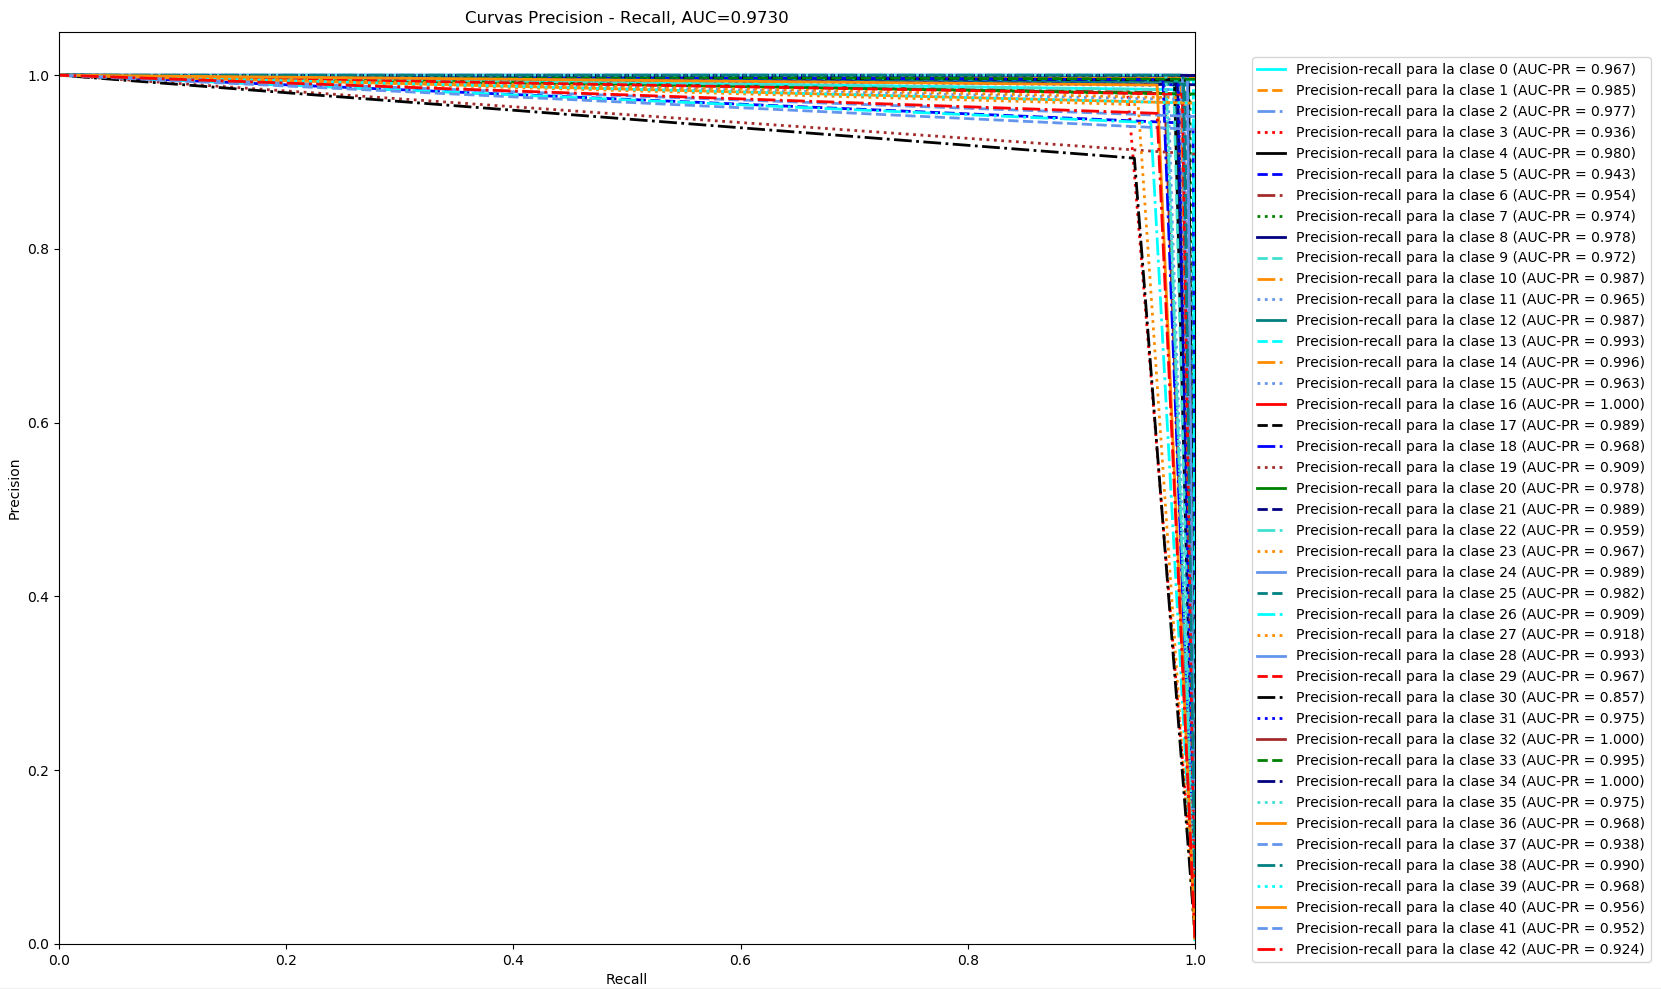
\includegraphics[width=\textwidth, height=0.7\textheight,keepaspectratio]{images/desarrollo/testResults/german/PR_curve_modelE} 
		%\end{center}
		\vspace{-1em}
		\begin{center}
		\caption{\tiny{Área debajo de la Curva PR del Modelo E - Dataset de imágenes de Alemania}}
		\vspace{-1em}
		{\tiny{Fuente: Elaboración propia}}
		\end{center}
		
	\end{figure}	
}



%------------------------------------------------------------------------------------------------------------------------------------------


\frame{
\begin{block}
{\Large{Resultados de la tesis - Señales de Tránsito de Perú}}
\end{block}
%\vskip 0.5cm

	\begin{table}[H]
			\begin{center}
			\caption{\small{Indicadores de los 5 modelos entrenados para el Dataset - Perú}}
			\setlength{\tabcolsep}{2pt}
			\begin{tabular}{|>{\tiny}c|>{\tiny}c|>{\tiny}c|>{\tiny}c|>{\tiny}c|>{\tiny}c|}
			\cline{1-6}
			 \textbf{Indicadores}    & \textbf{Modelo A(\%)} & \textbf{Modelo B(\%)} & \textbf{Modelo C(\%)} &\textbf{ Modelo D(\%)} & \textbf{Modelo E(\%)} \\ \hline
			\multicolumn{1}{|c|}{\textbf{\tiny PVP}}        & 95.78     & 97.61       & 98.21       & 98.09       & 98.81       \\ \hline
			\multicolumn{1}{|c|}{\textbf{\tiny PVN}}        & 99.44     & 99.69       & 99.75       & 99.69       & 99.83       \\ \hline
			\multicolumn{1}{|c|}{\textbf{\tiny PPV}}        & 96.75     & 98.29       & 98.51       & 98.04       & 98.94       \\ \hline
			\multicolumn{1}{|c|}{\textbf{\tiny AUC-PR}}     & 94.06     & 96.75       & 97.33       & 96.71       & 98.19       \\ \hline
			\multicolumn{1}{|c|}{\textbf{\tiny AUC-ROC}}    & 97.62     & 98.66       & 98.99       & 98.90       & 99.33       \\ \hline
			\multicolumn{1}{|c|}{\textbf{\tiny ACC}}        & 96.74     & 98.23       & 98.55       & 98.21       & 99.02       \\ \hline
			\end{tabular}
			\end{center}
			\begin{center}
				\vskip 0.2cm
				{\small{Fuente: Elaboración propia.}}
				\end{center}
		\end{table}
}



\frame{
\begin{block}
{\Large{Señales de Tránsito de Perú}}

\end{block}
%\vskip 0.5cm

	\begin{figure}[H]
		\begin{center}
		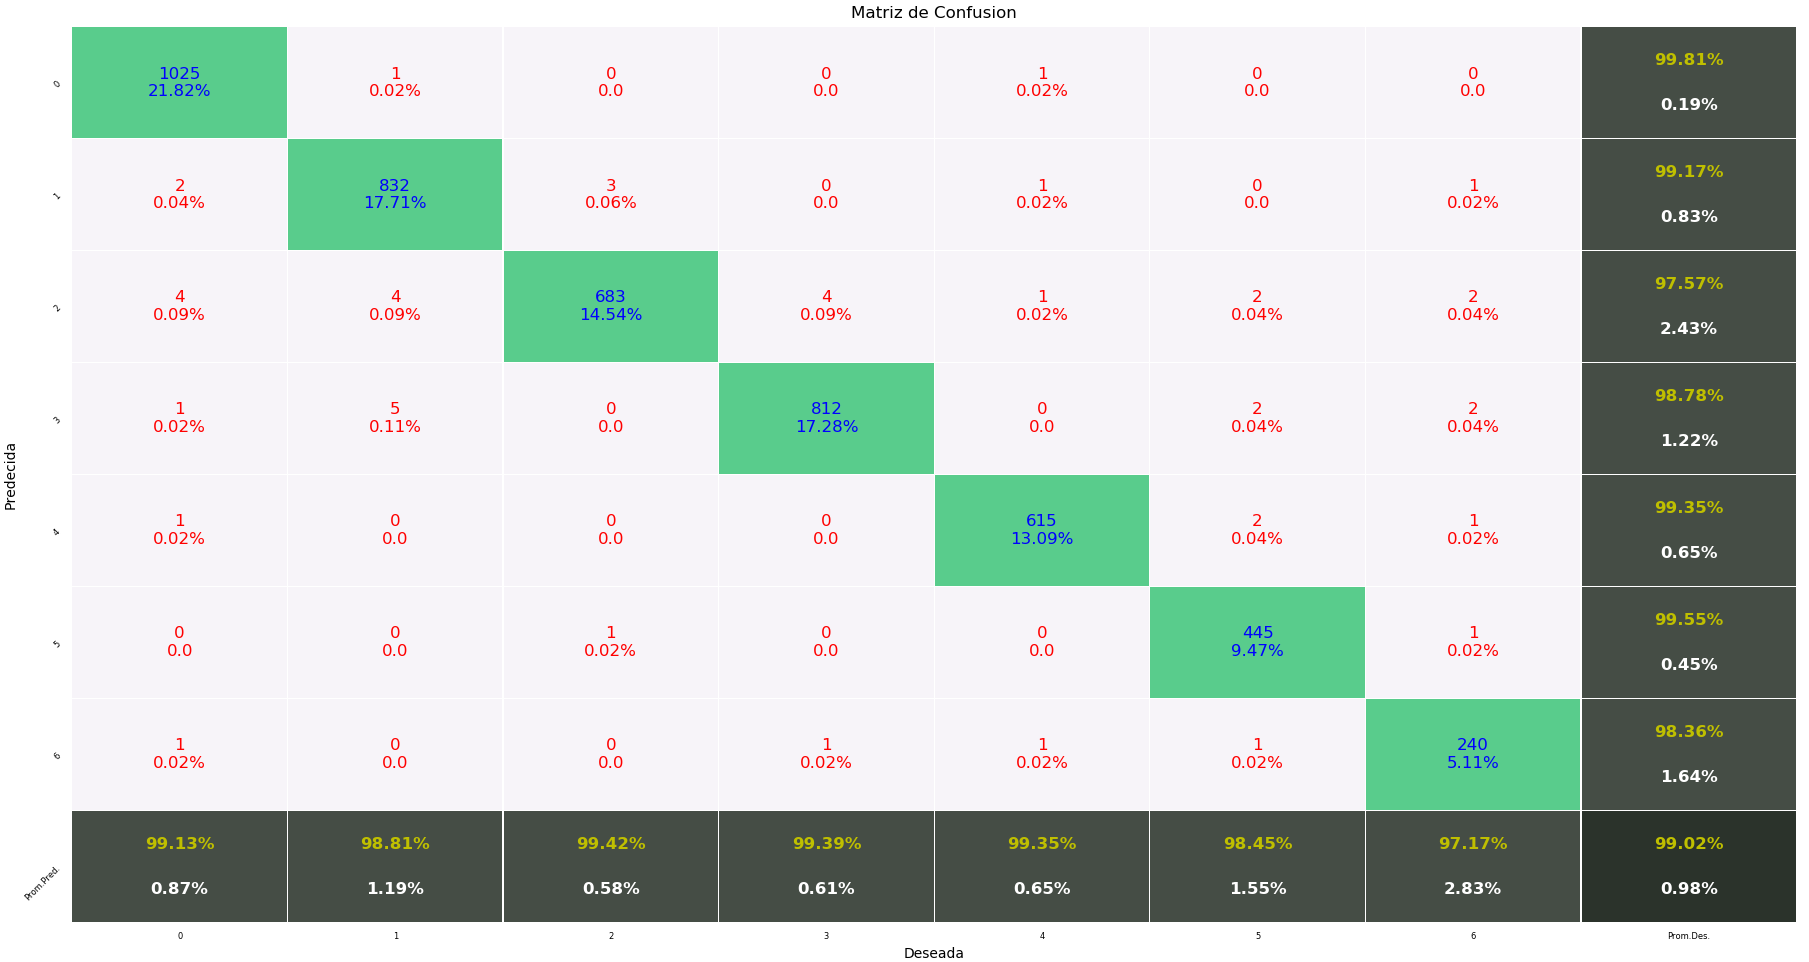
\includegraphics[width=\textwidth, height=0.7\textheight,keepaspectratio]{images/desarrollo/testResults/peru/modelE} 
		\end{center}
		\vspace{-1em}
		\begin{center}
		\caption{\tiny{Matriz de Confusión del Modelo E - Dataset de imágenes de Perú}}
		\vspace{-1em}
		{\tiny {Fuente: Elaboración propia}}
		\end{center}
		%\vspace{-1.5em}
	\end{figure}
}


\frame{
\begin{block}
{\Large{Señales de Tránsito de Perú}}

\end{block}
%\vskip 0.5cm
	\begin{figure}[H]
		\begin{center}
		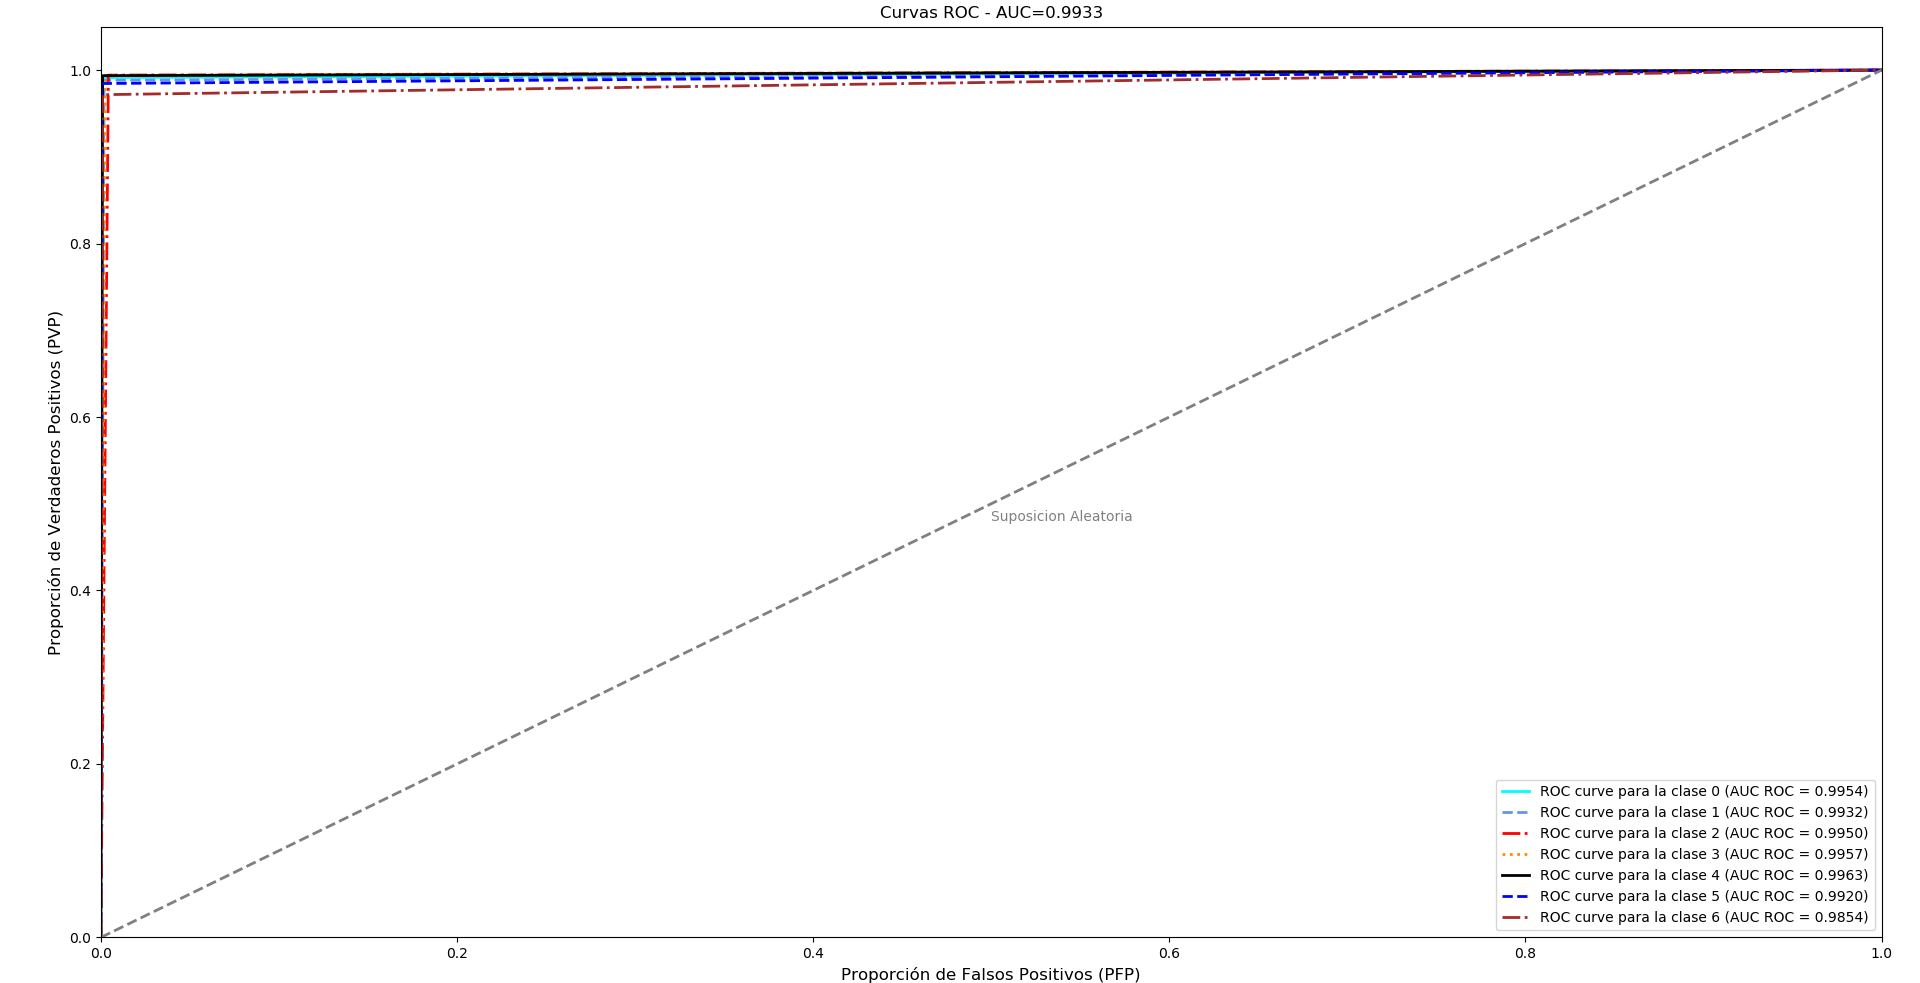
\includegraphics[width=\textwidth, height=0.7\textheight,keepaspectratio]{images/desarrollo/testResults/peru/ROC_curve_modelE} 
		\end{center}
		\vspace{-1em}
		\begin{center}
		\caption{\tiny{Área debajo de la Curva ROC del Modelo E - Dataset de imágenes de Perú}}
		\vspace{-1em}
		{\tiny {Fuente: Elaboración propia}}
		\end{center}
	\end{figure}
}

\frame{
\begin{block}
{\Large{Señales de Tránsito de Perú}}

\end{block}
%\vskip 0.5cm
	\begin{figure}[H]
		%\begin{center}
		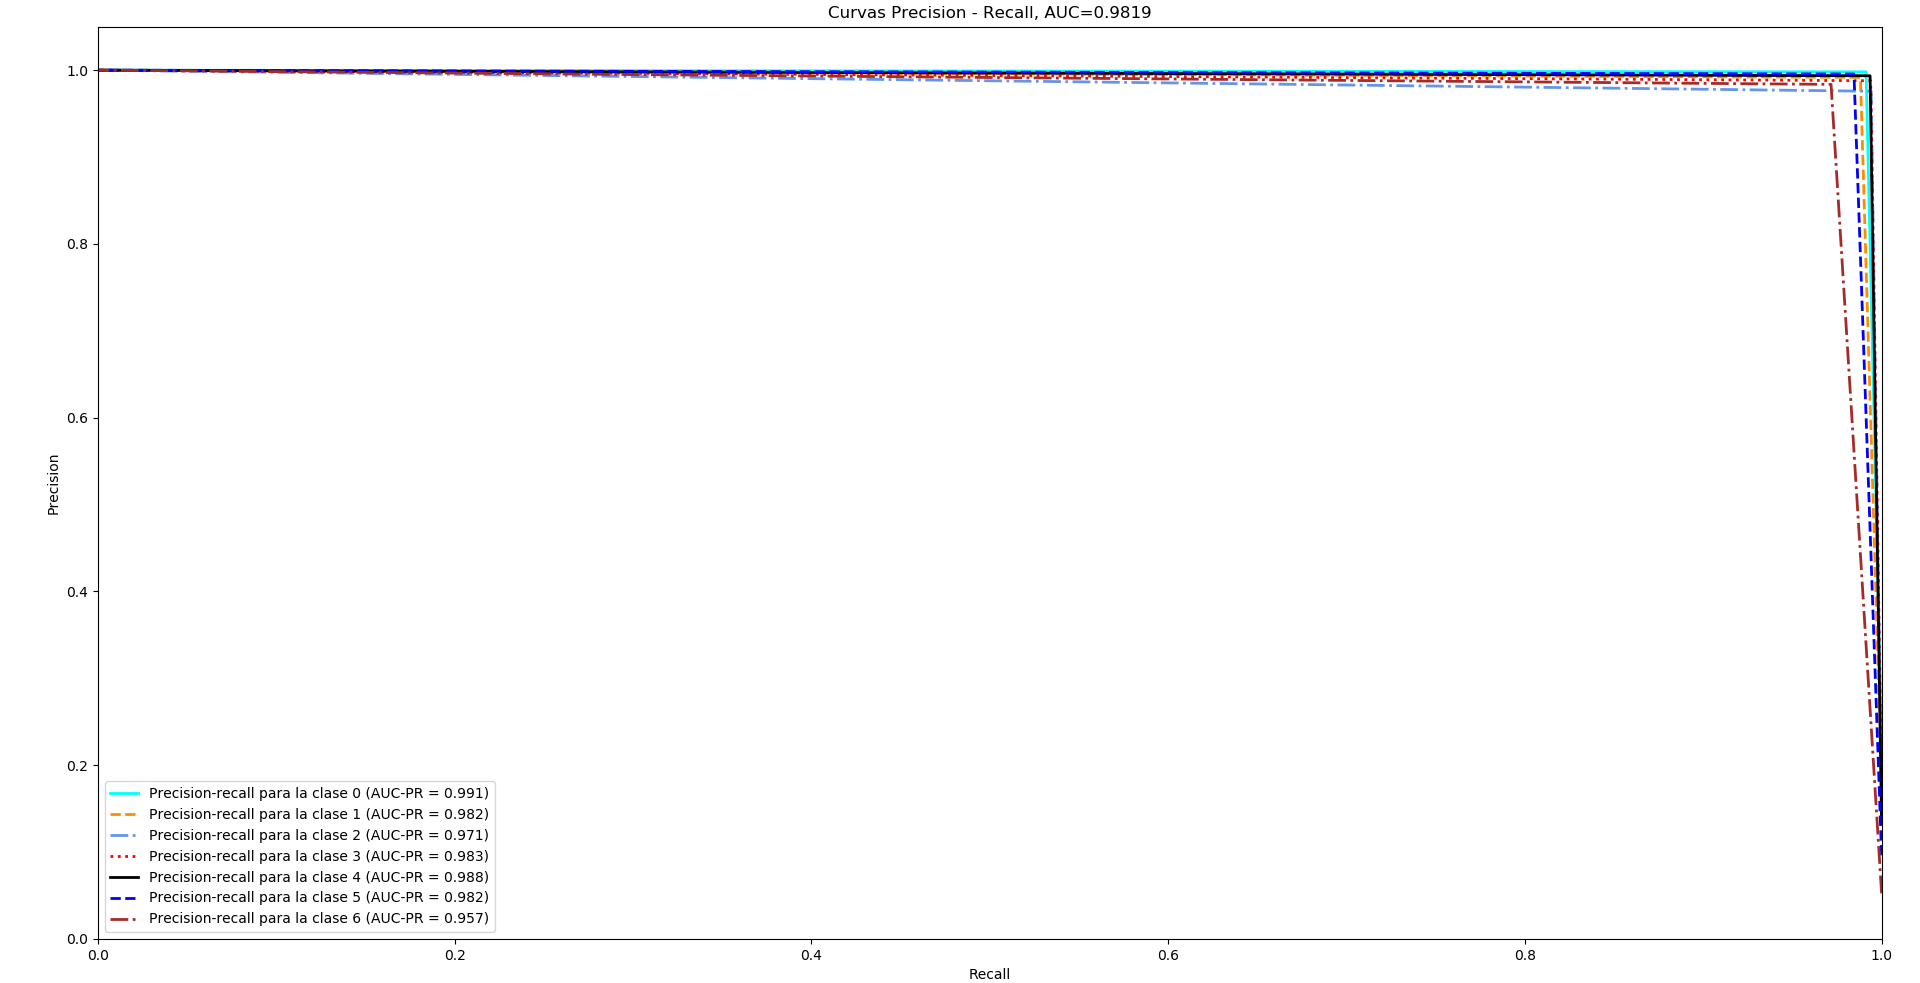
\includegraphics[width=\textwidth, height=0.7\textheight,keepaspectratio]{images/desarrollo/testResults/peru/PR_curve_modelE} 
		%\end{center}
		\vspace{-1em}
		\begin{center}
		\caption{\tiny{Área debajo de la Curva PR del Modelo E - Dataset de imágenes de Perú}}
		\vspace{-1em}
		{\tiny{Fuente: Elaboración propia}}
		\end{center}
		
	\end{figure}	
}



%------------------------------------------------------------------------------------------------------------------------------------------


\section{Consideraciones finales}


\frame{
\begin{block}
{\Large{Consideraciones finales}}
\end{block}
\vskip 0.3cm
	\begin{itemize}
		%Al finalizar la investigación podemos confirmar que se cumplieron los objetivos específicos planteados.
		\item<1-> {\bf Conclusiones:}
		\begin{itemize}
		\item<2-> Se obtuvo dos datasets de imágenes de señales de tránsito, uno de Alemania distribuidas en 43 categorías y otro de Perú distribuidas en 7 categorías, compuestos inicialmente por 51839 imágenes y 614 imágenes respectivamente.
		\vskip 0.25cm
		\item<3->Se analizaron los datasets y al dividirlos en 3 grupos (entrenamiento, validación y evaluación), se determinó la necesidad de aumentar ambos y esto fue realizado con la ayuda de técnicas de procesamiento de imágenes.
		\vskip 0.25cm
		\item<4->Fueron diseñados cinco modelos de red para cada dataset, los cuales fueron entrenados, validados y evaluados individualmente. 
		\vskip 0.25cm
		\item<5->Luego de experimentar el uso de diversas funciones de activación, funciones de costo, ajuste de parámetros y métodos de optimización, se logró determinar un conjunto de hiperparámetros (Sección 3.2) de los cuales solo la Tasa de Aprendizaje varía para cada dataset de imágenes.
	\end{itemize}
\end{itemize}
}

\frame{
\begin{block}
{\Large{Consideraciones finales}}
\end{block}
\vskip 0.3cm
	\begin{itemize}
		\item<1-> {\bf Conclusiones:}
		\begin{itemize}
		\item<2-> Al finalizar el análisis de los 10 modelos (cinco por cada dataset), se puede observar que cuanto más profunda sea la red neuronal, se obtienen mejores resultados. 
		\vskip 0.25cm
		\item<3->El modelo final obtenido compuesto principalmente de 4 capas convolucionales, 2 capas totalmente conectadas y un total de 90185 neuronas, contribuye en el reconocimiento de señales de Tránsito de Alemania con una tasa de acierto del {\bf 98.62\%}, mucho mejor que el resultado de 95.29\% obtenido por \cite{Ayuque2016} y mucho más próximo al mejor resultado de 99.46\% obtenido en las investigaciones hechas por \cite{Ciresan} en base al dataset GTSRB.
		\vskip 0.25cm
		\item<4->Para el dataset de señales de tránsito vehicular del Perú, el modelo E con el mismo diseño neuronal y similares configuraciones compuesto por 279623 neuronas permite también obtener un {\bf alto grado de acierto (99.02\%)} tras analizar 4698 imágenes. 
	\end{itemize}
\end{itemize}
}

\frame{
\begin{block}
{\Large{Consideraciones finales}}
\end{block}
\vskip 0.3cm
	\begin{itemize}
		\item<1-> En conclusión, el objetivo general que trata sobre implementar un modelo basado en el aprendizaje profundo de redes neuronales convolucionales para reconocer automáticamente señales de tránsito vehicular fue conseguido a través del Modelo E.	
	\end{itemize}
}


\frame{
\begin{block}
{\Large{Consideraciones finales}}
\end{block}
\vskip 0.5cm
	\begin{itemize}
		\item<1-> {\bf  Trabajos futuros:}
		\begin{itemize}
		\item<2->El modelo puede ser mejorado(ampliado), teniendo muchas más capas convolucionales y capas totalmente conectadas para poder experimentar si existe o no alguna mejora en los resultados. Además, se recomienda obtener muchas más imágenes para exceder el rendimiento humano, \citep{Goodfellow-et-al-2016}
		\vskip 0.3cm
		\item<3->El dataset de señales de tránsito del Perú también puede ser ampliado con la finalidad de abarcar más categorías, ya que se tiene confianza por lo mostrado con el dataset de Alemania que el modelo es robusto para soportar mayor cantidad de estas.
		\vskip 0.3cm
		\item<4->Se sugiere integrar el modelo obtenido en un sistema más general que primero localice las señales de tránsito en escenas que abarcan más de una señal de tránsito, para luego proceder a su multireconocimiento.
		\end{itemize}
\end{itemize}
}

